\documentclass[letterpaper,11pt]{article}
\usepackage{cmap}
\usepackage[T1]{fontenc}
\usepackage[margin=0.75in]{geometry}
\usepackage{amsmath,amssymb}
\usepackage{graphicx}
\usepackage{booktabs}
\usepackage{longtable}
\usepackage{float}
\usepackage{setspace}
\usepackage{ragged2e}
\usepackage[numbers,sort&compress]{natbib}
\usepackage{hyperref}
\hypersetup{colorlinks=true,allcolors=black}
\usepackage{etoolbox}
\usepackage{xcolor}
\usepackage{soul}
\usepackage{caption}
\usepackage{authblk}
\usepackage{titlesec}
\usepackage[left,modulo]{lineno}
\usepackage{textcomp}
\usepackage{upgreek}
% Labels: \(\upalpha\) helix, C\(\upalpha\); variables: \(\chi_1\).

\captionsetup{font=normalsize,justification=justified}
\onehalfspacing
% Left-aligned body text, retaining the article first-line indentation.
\setlength{\RaggedRightParindent}{\parindent}
\AtBeginDocument{\RaggedRight}

\setcounter{secnumdepth}{3}
\titleformat{\section}{\normalfont\bfseries\normalsize}{}{0pt}{}
\titleformat{\subsection}{\normalfont\bfseries\normalsize}{}{0pt}{}
\titleformat{\subsubsection}{\normalfont\bfseries\normalsize}{}{0pt}{}
\renewcommand{\Authfont}{\normalfont\normalsize}
\renewcommand{\Affilfont}{\normalfont\normalsize}

\title{Scientific Manuscript Template and Style Demonstration}
\author[1]{First Author}
\author[2]{Second Author}
\author[1,*]{Corresponding Author}
\affil[1]{Department of Example Studies, Example University, City, Country}
\affil[2]{Institute of Demonstration Research, Example University, City, Country}
\date{*Correspondence: author@example.edu}

\begin{document}
\modulolinenumbers[1]
\linenumbers
\maketitle

\begin{abstract}
This document serves as an authoring template and structural reference for scientific manuscripts. It demonstrates the complete set of supported editorial elements, including structured front matter, typographic styling, revision markup commands, inline and display mathematics, figure insertion, publication-quality tables, and bibliographic citation management. Authors can replace this sample content with their domain-specific narrative while preserving the underlying formatting standards.
\end{abstract}

\section{Introduction}

The introduction establishes research motivation, outlines background literature, and states specific aims. This template illustrates each document element and its operational importance within the authoring workflow.

\subsection{Typographic Formatting and Scientific Notation}
Standard prose supports core typographic variations to convey emphasis and semantic distinction:
\begin{itemize}
  \item \textbf{Bold text} is used for key terms, panel identifiers, and lead-in headings.
  \item \textit{Italic text} is reserved for gene names, foreign phrases, and variable symbols.
  \item Monospace \texttt{code text} identifies filenames, commands, or code identifiers.
  \item Scientific units and coordinates should remain formatted with non-breaking spaces, such as $15$~\AA\ distances, $10~\upmu\text{M}$ concentrations, and directional $5^\prime$ and $3^\prime$ ends.
\end{itemize}

\subsection{Collaborative Colour Markup}
To streamline editorial revisions among co-authors, the same colour commands work in main and supplementary documents. Colours indicate presentation, not who wrote or accepted the text:
\begin{itemize}
  \item \textbf{New Data:} Use \verb|\textcolor{red}{...}| to highlight newly inserted findings, for example: \textcolor{red}{This sentence highlights updated measurements added during revision.}
  \item \textbf{Editorial Remarks:} Use \verb|\textcolor{blue}{...}| for an explicitly chosen blue passage: \textcolor{blue}{Verify that sample controls are fully documented.}
  \item \textbf{Text Highlights:} Use \verb|\hl{...}| to spotlight specific text passages: \hl{This passage represents a key take-away message.}
\end{itemize}

\begingroup\color{red}
Use a scoped red group for several paragraphs of marked text.

Each paragraph remains separately editable in Aspyrus.
\endgroup

\begingroup\color{blue}
Use a scoped blue group when the exchange calls for blue text.
\endgroup


\section{Results}

The results section reports experimental observations and computational analyses supported by quantitative figures and tables.

\subsection{Mathematical Formulations}
Inline mathematical notation such as variables $x$, $y$, and parameter $\alpha$ integrate directly within running text. Display equations should be declared within standard equation environments to provide automated numbering and labels for in-text referencing:
\begin{equation}\label{eq:linear}
y = f(x) = \alpha x + \beta
\end{equation}
where $\alpha$ denotes the slope parameter and $\beta$ represents the baseline intercept. Numbered equations can be referenced in the text using Eq.~\eqref{eq:linear}.

\subsection{Figure Environments and Relative Paths}
Figures are authored using standard \verb|\begin{figure}| environments. The file path points symmetrically to the main figure directory at \texttt{../assets/figures/main/}:

\begin{figure}[htbp]
  \centering
  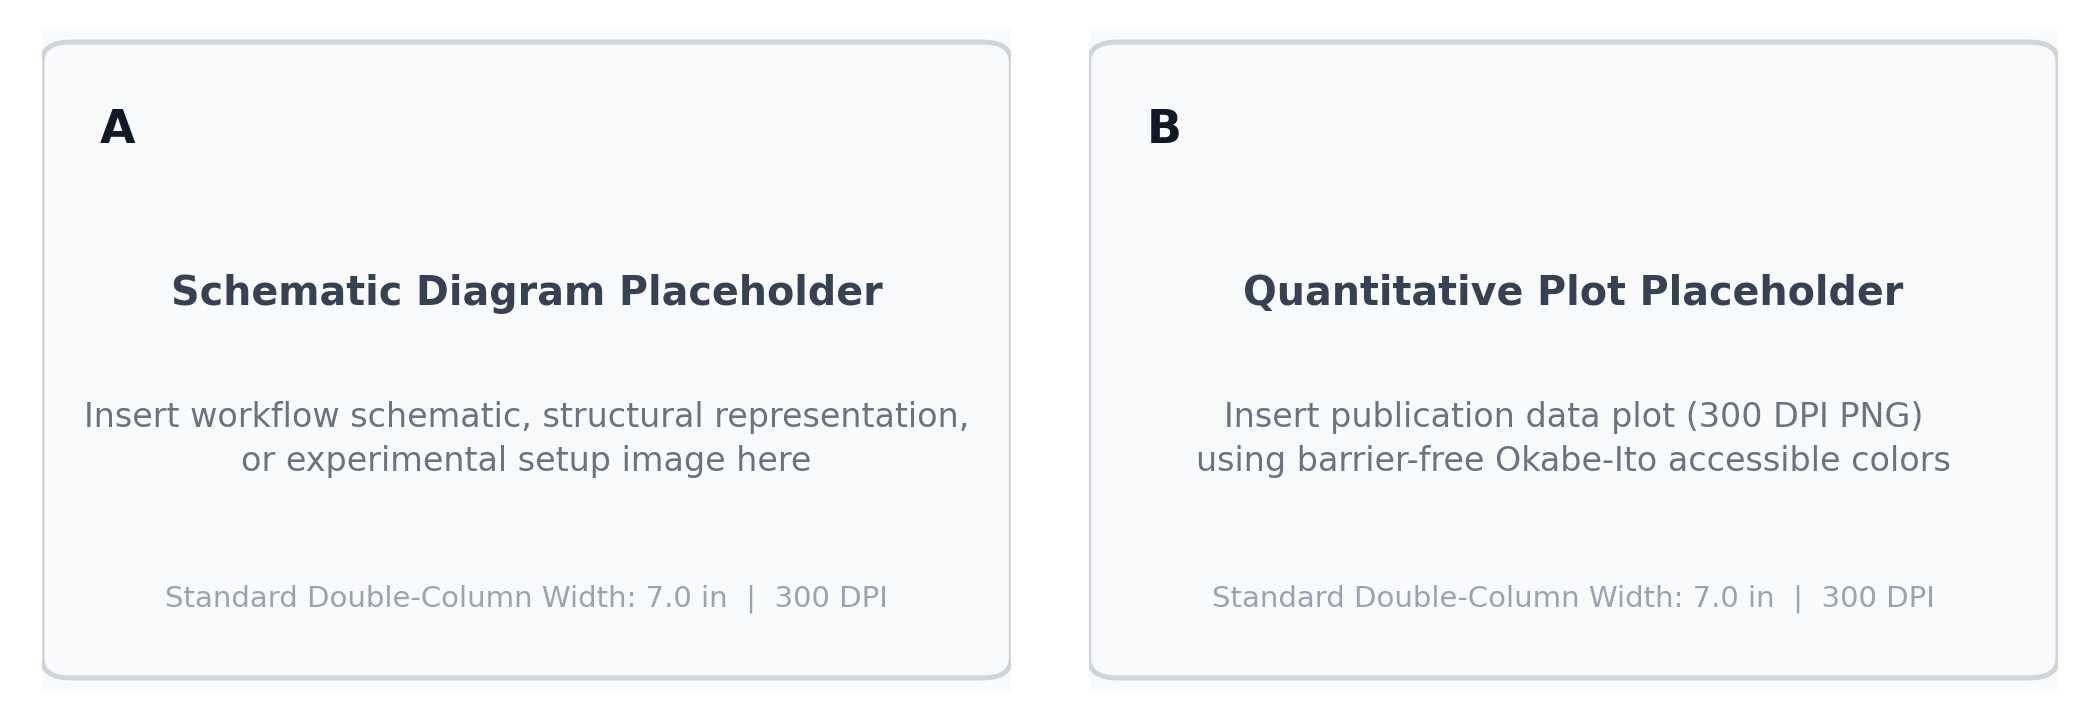
\includegraphics[width=\textwidth,keepaspectratio]{../assets/figures/main/figure1.png}
  \caption{\textbf{Template demonstration of multi-panel figure layout.} 
  \textbf{(A)} Placeholder for schematic diagrams, experimental workflows, or structural representations. 
  \textbf{(B)} Placeholder for quantitative plots, titration curves, or statistical distributions formatted at 300 DPI.}
  \label{fig:example}
\end{figure}

As shown in Figure~\ref{fig:example}, sub-panels are designated with bold capital letters \textbf{(A)} and \textbf{(B)} to guide the reader.

\subsection{Publication Tables}
Tables should follow professional publication standards using the \texttt{booktabs} package, avoiding vertical rules and employing \verb|\toprule|, \verb|\midrule|, and \verb|\bottomrule|:

\begin{table}[htbp]
  \centering
  \caption{\textbf{Example summary table illustrating clean horizontal booktabs layout.}}
  \label{tab:example}
  \begin{tabular}{lccc}
    \toprule
    \textbf{Sample Identifier} & \textbf{Measurement A} & \textbf{Measurement B} & \textbf{Validation Status} \\
    \midrule
    Sample 1 & $10.5 \pm 0.2$ & $1.25$ & Pass \\
    Sample 2 & $20.1 \pm 0.4$ & $2.50$ & Pass \\
    Sample 3 & $35.8 \pm 0.6$ & $4.10$ & Review \\
    \bottomrule
  \end{tabular}
\end{table}

Table~\ref{tab:example} presents structured measurement summaries with explicit parameter units.

\section{Discussion}

The discussion contextualizes findings relative to established benchmarks and literature precedents \cite{sample2024, reference2023}. Authors can cite individual or grouped references using the standard \verb|\cite{...}| macro. The bibliography is aggregated automatically from atomic records located in the \texttt{references/bib/} folder.

\section{Methods}

\subsection{Computational Implementation}
This section details software tools, algorithms, and simulation parameters. All reproducible data files and standalone tables are organized under \texttt{assets/tables/}.

\subsection{Asset and Provenance Tracking}
Project assets, including Figure~\ref{fig:example} and Table~\ref{tab:example}, are mapped in \texttt{assets/assets.csv} to maintain provenance between computational workflows and final publication assets.

\bibliographystyle{unsrtnat}
\bibliography{../references/references}

\end{document}
